\chapter{Physikalischer Hintergrund}
%
\section{Standardmodell der Teilchenphysik}
%
Das Standardmodell (SM) der Teilchenphysik beschreibt den Aufbau der Materie, sowie ihre Wechselwirkung auf elementarer Ebene. Sie stellt eine seit vielen Jahrzehnten bestehende und damit vielfältig getestete Theorie dar und unterliegt auch heute weiter regelmäßigen Tests. Allgemein werden zunächst zwei Arten von Teilchen unterschieden: Fermionen (halbzahliger Spin $s=\sfrac{\hbar}{2}$)($\hbar$: reduziertes Plancksches Wirkungsquantum) und Bosonen (ganzzaliger Spin $s=\hbar$). Die Fermionen nach dem Standardmodell sind in drei Generationen von Quarks, sowie drei Generationen von Leptonen unterteilt, wie sie unten aufgeführt sind. Die Leptonengenerationen bestehen hierbei aus einem ganzzahlig (in Einheiten der Elementarladung) geladenen punktförmigen Lepton ($e$, $\mu$, $\tau$), sowie den dazugehörigen Neutrinos $\nu_e$, $\nu_\mu$, $\nu_\tau$.
%
\begin{figure}
  \centering
      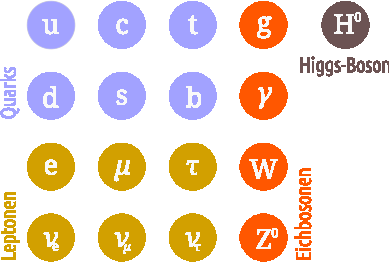
\includegraphics[width=0.6\textwidth]{content/SM.pdf}
  \caption{Die Elementarteilchen im Stadardmodell der Teilchenphysik.}
\end{figure}
%
Auch die Quarks gliedern sich in drei Generationen. Diese erfolgt über die Eigenschaften der Teilchen: die Quarks lassen sich in \textit{up-artige} Quarks mit Ladung $\sfrac{2}{3}$, sowie \textit{down-artige} mit Ladung $\sfrac{-1}{3}$ einteilen. Es gilt für diese Darstellung dass die Teilchenmassen zwischen den Generationen von links nach rechts zunehmen.\\
Im Standardmodell unterscheidet man zwischen drei Wechselwirkungen der Elementarteilchen untereinander: die starke Wechselwrikung zwischen farbgeladenen Teilchen, die schwache Wechselwirkung an welcher alle Elementarteilchen teilnehmen, sowie die elektromagetische Wechselwirkung, welcher nur elektrisch geladene Teilchen unterliegen. Die letzten beiden lassen sich im Rahmen des SM zur elektroschwachen Wechselwirkung vereinigen.
Die Farbladung in der starken Wechselwirkung beschreibt das Konzept einer Quantenzahl deren Existenz zur theoretischen Umsetzung des sogenannten \textit{confinement} dient. \textit{confinement} meint hierbei die Tatsache, dass alle elementaren Teilnehmer der starken Wechselwirkung nur in "farbneutralen" (z.B. Farbe + Antifarbe) Zuständen frei existieren; freie Quarks lassen sich, da sie eine von null verschiedene Farbladung tragen also nicht beobachten.\\
%
Die Übertragung der Wechselwirkungen findet über die oben genannten Bosonen statt. Bei der starken Wechselwirkung sind dies die acht verschiedenen Gluonen ($g$). Sie tragen eine Farbladung und einen ganzzahligen Spin $\hbar$. Die Austauschteilchen der elektroschwachen Wechselwirkung sind die Photonen ($\gamma$) für den elektromagnetischen Teil, sowie für die schwache Wechselwirkung das neutrale $\symup{Z}$-Boson und die geladenen $\symup{W^{\pm}}$-Bosonen. \\
%
Aus den oben aufgeführten Quarks existieren über Kombination mehrere so genannte Hadronen - also über Resonanz aus Quarks zusammengesetzte Teilchen. Hierbei unterscheidet man die aus Quark und Antiquark bestehenden Mesonen und die aus drei Quarks bestehenden Baryonen. Zu den Mesonen zählt beispielsweise auch das $J/\!\symup{\Psi}$, während das Proton ein prominenter Vertreter der Baryonen ist.
